% Provenance (never printed): cycle 4 SVT/physique, "La planete Terre,
% l'environnement": uneven heating of the Earth, movements of the
% atmosphere, the global circulation and the climate zones; see
% sources/book1/PROVENANCE.md. Book 1, grade 8, chapter 2.
% Vocabulary guard: owns convection cell (atmospheric, descriptive), sea
% breeze and land breeze, the global winds, the global circulation. The
% Coriolis effect is told as "the Earth's rotation deflects"; Hadley and
% Ferrel cells and the intertropical convergence zone are named in prose
% only (Book 3 owns them); mantle convection is Book 2's.
\chapter{पवनें और वैश्विक परिसंचरण}\label{ch:g8:winds-global-circulation}

सदियों तक, यूरोप और अफ़्रीका के बंदरगाहों से अमेरिका महाद्वीपों की ओर निकलने वाले
पाल-जहाज़ पूर्व से आने वाली एक स्थिर पवन पर भरोसा करते थे, जो \omterm{def:g3:continents-and-oceans:equator}{भूमध्य रेखा} के दोनों
ओर बहती है और उन्हें अटलांटिक के पार ले जाती थी। दुनिया भर के नाविक उसे जानते थे, और
अमेरिका महाद्वीपों के साथ शुरुआती व्यापार उसी पर टिका था: वह \emph{व्यापारिक पवन}
है। आज भी मालवाहक जहाज़ अपनी यात्राएँ छोटी करने के लिए \omterm{def:g8:winds-global-circulation:global-winds}{व्यापारिक पवनों} का, और उनसे
चलने वाली महासागरीय धाराओं का, उपयोग करते हैं।
% ledger: nos:trade-winds

\begin{omfigure}
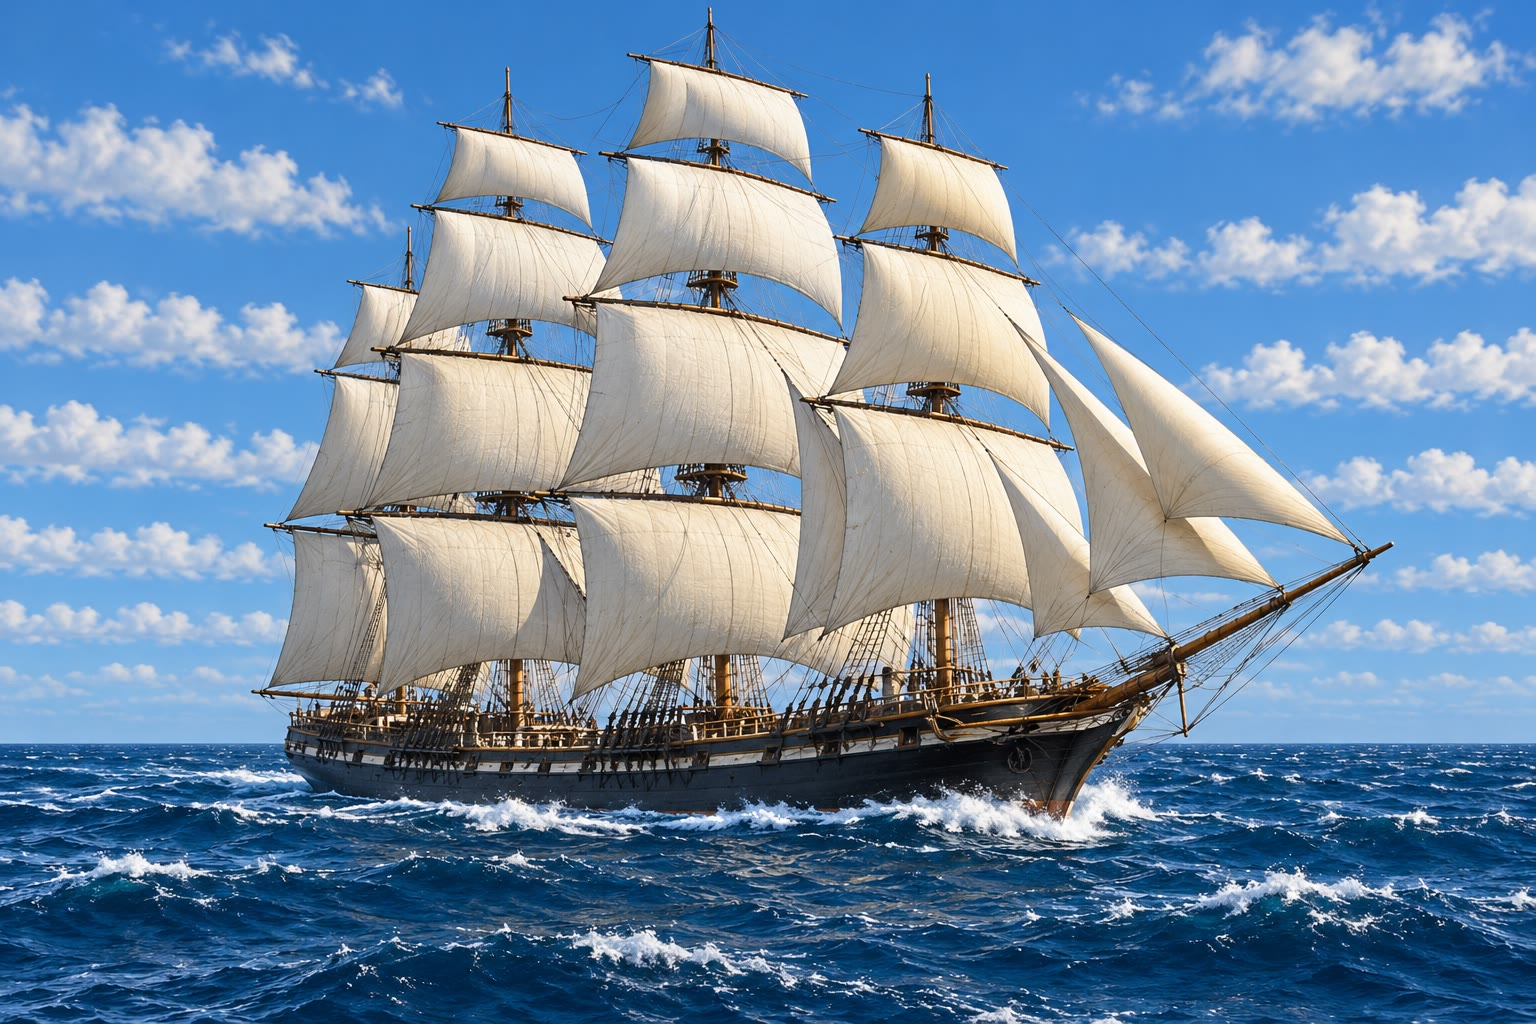
\includegraphics[width=0.62\linewidth]{images/book1/ai/g8-sailing-ship.jpg}

{\small खुले \omterm{def:g2:water-on-earth:ocean}{महासागर} पर एक स्थिर पवन के आगे-आगे चलता एक पाल-जहाज़ (एक सामान्य दृश्य
का AI चित्रण)।}
\label{fig:g8:winds-global-circulation:ship}
\end{omfigure}

व्यापारिक पवन पूर्व से क्यों बहती है, और हमेशा उन्हीं जगहों पर क्यों? \omterm{def:g5:weather-and-climate:tropics}{कर्क और मकर
रेखाओं} के पास \omterm{def:g5:weather-and-climate:desert}{मरुस्थल} और \omterm{def:g3:continents-and-oceans:equator}{भूमध्य रेखा} के पास \omterm{def:g5:weather-and-climate:rainforest}{वर्षावन} क्यों हैं? जवाब सूर्य से शुरू
होता है।

\begin{recall}
पवन चलती हुई हवा है (भौतिकी की किताबें)। हवा हर उस चीज़ पर दबाव डालती है जिसे वह
छूती है, और ऊँचाई के साथ दाब घटता है (\cref{ch:g8:the-atmosphere})। \omterm{def:g1:watching-the-weather:weather}{मौसम}
\omterm{def:g8:the-atmosphere:layers}{क्षोभमंडल} में होता है, जो वायुमंडल की सबसे निचली परत है। पृथ्वी के \omterm{def:g5:weather-and-climate:climate}{जलवायु} क्षेत्र
हैं: \omterm{def:g3:continents-and-oceans:equator}{भूमध्य रेखा} के पास गरम और नम, \omterm{def:g5:weather-and-climate:rainforest}{वर्षावनों} के साथ; \omterm{def:g5:weather-and-climate:tropics}{कर्क और मकर रेखाओं} के पास गरम
और सूखे \omterm{def:g5:weather-and-climate:desert}{मरुस्थल}; \omterm{def:g3:continents-and-oceans:poles}{ध्रुवों} की ओर शीतोष्ण, फिर ठंडे क्षेत्र
(\cref{ch:g5:weather-and-climate})।
\end{recall}

\section{सूर्य पृथ्वी को असमान रूप से गरम करता है}

किसी विषुव के दिन दोपहर को सूर्य \omterm{def:g3:continents-and-oceans:equator}{भूमध्य रेखा} पर ठीक सिर के ऊपर होता है। वहाँ उसकी
किरणें खड़ी आती हैं और ज़मीन के एक छोटे टुकड़े पर पड़ती हैं। और उत्तर या दक्षिण में वही
किरणें तिरछी आती हैं और एक बड़े टुकड़े पर फैल जाती हैं: हर वर्ग मीटर को उनकी ऊर्जा
कम मिलती है। \ang{60} \omterm{def:g6:latitude-longitude:latitude}{अक्षांश} पर वही पुंज \omterm{def:g3:continents-and-oceans:equator}{भूमध्य रेखा} की तुलना में दोगुनी ज़मीन ढकता
है, इसलिए हर वर्ग मीटर को आधी ऊर्जा मिलती
है।
% ledger: (geometry: figdata/grade-8/sunlight_spread.py, spread = 1/cos(latitude))

\begin{omfigure}
\begin{tikzpicture}[font=\footnotesize]
  \def\R{2.6}\def\w{0.2}
  \fill[blue!10] (0,0) circle (\R);
  \draw (0,0) circle (\R);
  \draw[black!50] (-\R,0) -- (\R,0);
  \draw[black!40, dashed] (0,0) -- (60:\R);
  \draw[black!40] (0,0) ++(0:0.7) arc (0:60:0.7);
  \node at (25:0.95) {\ang{60}};
  \node[anchor=east, black!60] at (-\R-0.05,0) {भूमध्य रेखा};
  % beam at the equator: rays between y = -w and y = w
  \foreach \y in {-0.2,-0.1,0,0.1,0.2} {
    \pgfmathsetmacro{\x}{sqrt(\R*\R-\y*\y)}
    \draw[orange!80!black, -{Stealth[length=1.6mm]}] (6.2,\y) -- (\x+0.03,\y);}
  \draw[omThm, line width=2.2pt] ({sqrt(\R*\R-0.35*0.35)},-0.35) arc ({asin(-\w/\R)}:{asin(\w/\R)}:\R);
  % beam near 60 degrees: rays between y = R sin 60 - w and + w
  \pgfmathsetmacro{\yc}{\R*sin(60)}
  \foreach \d in {-0.2,-0.1,0,0.1,0.2} {
    \pgfmathsetmacro{\y}{\yc+\d}
    \pgfmathsetmacro{\x}{sqrt(\R*\R-\y*\y)}
    \draw[orange!80!black, -{Stealth[length=1.6mm]}] (6.2,\y) -- (\x+0.03,\y);}
  \draw[omThm, line width=2.2pt] ({sqrt(\R*\R-(\yc-\w)^2)},\yc-\w) arc ({asin((\yc-\w)/\R)}:{asin((\yc+\w)/\R)}:\R);
  \node[anchor=west, align=left] at (6.3,0) {वही पुंज\\एक छोटे टुकड़े पर};
  \node[anchor=west, align=left] at (6.3,\yc) {वही पुंज फैला हुआ\\दोगुनी ज़मीन पर};
\end{tikzpicture}

{\small किसी विषुव के दिन दोपहर को सूर्य के प्रकाश के दो एक जैसे पुंज। \omterm{def:g3:continents-and-oceans:equator}{भूमध्य रेखा} पर
वे सीधे नीचे एक छोटे टुकड़े पर पड़ते हैं (मोटी रेखा); \ang{60} \omterm{def:g6:latitude-longitude:latitude}{अक्षांश} पर वे तिरछे
पड़ते हैं और दोगुनी ज़मीन ढकते हैं।}
% ledger: (geometry: figdata/grade-8/sunlight_spread.py)
\label{fig:g8:winds-global-circulation:beams}
\end{omfigure}

\begin{center}\small
\begin{tabular}{|l|c|c|c|c|c|}
\hline
\omterm{def:g6:latitude-longitude:latitude}{अक्षांश} & \ang{0} & \ang{30} & \ang{45} & \ang{60} & \ang{75} \\
\hline
उसी पुंज से ढकी ज़मीन & 1 & 1.15 & 1.41 & 2 & 3.86 \\
\hline
प्रति वर्ग मीटर ऊर्जा (\omterm{def:g3:continents-and-oceans:equator}{भूमध्य रेखा} की ऊर्जा का \%) & 100 & 87 & 71 & 50 & 26 \\
\hline
\end{tabular}
\end{center}
% ledger: (figdata/grade-8/sunlight_spread.py main table)

सूर्य की परिक्रमा करते हुए पृथ्वी की झुकी हुई धुरी सिर के ऊपर वाले सूर्य को \omterm{def:g5:weather-and-climate:tropics}{कर्क और
मकर रेखाओं} के बीच आगे-पीछे ले जाती है, जिससे ऋतुएँ बनती हैं (भौतिकी की किताबें);
पर पूरे वर्ष \omterm{def:g3:continents-and-oceans:equator}{भूमध्य रेखा} के पास के क्षेत्रों को \omterm{def:g3:continents-and-oceans:poles}{ध्रुवों} के पास के क्षेत्रों से कहीं
ज़्यादा ऊर्जा मिलती है। यह असमान गरमाहट पवनों की मुख्य चालक है: वायुमंडल गरम हवा को
\omterm{def:g3:continents-and-oceans:poles}{ध्रुवों} की ओर और ठंडी हवा को \omterm{def:g3:continents-and-oceans:equator}{भूमध्य रेखा} की ओर ले जाता
है।
% ledger: mo:global-circ

\section{ऊपर उठती और नीचे उतरती हवा}

गरम हवा ठंडी हवा से हल्की होती है: वह ऊपर उठती है, और आसपास की ठंडी हवा उसकी जगह
लेने बहकर आती है। जहाँ हवा ऊपर उठती है, वहाँ वह ज़मीन पर कम दबाती है: वहाँ दाब
निम्न होता है। जहाँ हवा नीचे उतरती है, वहाँ वह ज़्यादा दबाती है: दाब उच्च होता है।
ज़मीन पर पवन उच्च दाब से निम्न दाब की ओर बहती है। ऊपर उठती, ठंडी होती, नीचे उतरती
और वापस बहती हुई हवा एक चक्कर में घूमती
है।
% ledger: jetstream:sea-breeze, mo:three-cells

\begin{definition}[संवहन कोष्ठ]\label{def:g8:winds-global-circulation:convection-cell}
वायुमंडल में \emph{संवहन कोष्ठ}\index{संवहन कोष्ठ} चलती हवा का एक चक्कर है: नीचे
से गरम हुई हवा ऊपर उठती है, ऊँचाई पर फैलती है, ठंडी होकर कहीं और नीचे उतरती है, और
ज़मीन के साथ-साथ वापस वहीं बहती है जहाँ से वह उठी थी। ऊपर उठती हवा के नीचे दाब निम्न
होता है; नीचे उतरती हवा के नीचे वह उच्च
होता है।
\end{definition}
% ledger: jetstream:sea-breeze, mo:three-cells

\begin{inthelab}[गरम हवा ऊपर उठती है]
घर के अंदर, पतले काग़ज़ की एक शीट से सेब के छिलके जैसा एक सर्पिल काटो, और उसे उसके
बीच से एक धागे पर लटकाओ। जाड़े में उसे किसी गरम रेडिएटर से काफ़ी ऊपर पकड़ो (कभी किसी
लौ या मोमबत्ती के ऊपर नहीं): वह धीरे-धीरे घूमने लगता है। रेडिएटर से गरम हुई हवा ऊपर
उठती है और सर्पिल को धकेलती है। उसे किसी ठंडी खिड़की के पास पकड़ो: क्या वह उलटी
दिशा में घूमता है, या बिल्कुल नहीं?
\end{inthelab}

सबसे छोटे \omterm{def:g8:winds-global-circulation:convection-cell}{संवहन कोष्ठ} धूप वाले दिन \omterm{def:g2:water-on-earth:ocean}{समुद्र} के किनारे महसूस किए जा सकते हैं। ज़मीन और
\omterm{def:g2:water-on-earth:ocean}{समुद्र} को एक जैसी धूप मिलती है, पर सूर्य की किरणें ज़मीन में गहरे नहीं जातीं, जबकि
\omterm{def:g2:water-on-earth:ocean}{समुद्र} अपनी ऊष्मा पानी की एक मोटी परत में फैला देता है। इसलिए दिन में ज़मीन कहीं
ज़्यादा गरम होती है, और रात में कहीं ज़्यादा ठंडी
होती है।
% ledger: jetstream:sea-breeze

\begin{omfigure}
\begin{tikzpicture}[font=\footnotesize, >={Stealth[length=2mm]}]
  \foreach \px/\title/\dir in {0/{दिन में: समुद्र समीर}/1, 8.3/{रात में: स्थल समीर}/-1} {
    \begin{scope}[xshift=\px cm]
      \fill[omSea] (0,0) rectangle (3.5,0.45);
      \fill[omLithAlluv] (3.5,0) -- (3.5,0.45) -- (7,0.75) -- (7,0) -- cycle;
      \draw (0,0.45) -- (3.5,0.45) -- (7,0.75);
      \node[anchor=south] at (3.5,3.25) {\textbf{\title}};
      \node at (1.75,0.22) {समुद्र};
      \node at (5.6,0.3) {ज़मीन};
    \end{scope}}
  % day loop: surface sea -> land, rise over land, return aloft, sink over sea
  \draw[->, omDef, line width=1.1pt] (1.2,0.8) -- (5.2,0.95);
  \draw[->, omThm, line width=1.1pt] (5.8,1.1) -- (5.8,2.4);
  \draw[->, black!60, line width=1.1pt] (5.2,2.75) -- (1.2,2.75);
  \draw[->, omDef, line width=1.1pt] (0.6,2.4) -- (0.6,1.1);
  \node[omDef] at (3.2,1.25) {समुद्र समीर};
  \node at (0.6,0.75) {\textbf{उच्च}};
  \node at (5.8,0.95) {\textbf{निम्न}};
  \fill[yellow!80!orange] (6.6,2.7) circle (0.25);
  \node[anchor=north, align=center] at (1.75,-0.1) {ठंडा समुद्र};
  \node[anchor=north, align=center] at (5.3,-0.1) {गरम ज़मीन};
  % night loop: surface land -> sea, rise over sea, return aloft, sink over land
  \begin{scope}[xshift=8.3cm]
    \draw[->, omDef, line width=1.1pt] (5.2,1.0) -- (1.2,0.8);
    \draw[->, omThm, line width=1.1pt] (0.6,1.1) -- (0.6,2.4);
    \draw[->, black!60, line width=1.1pt] (1.2,2.75) -- (5.2,2.75);
    \draw[->, omDef, line width=1.1pt] (5.8,2.4) -- (5.8,1.15);
    \node[omDef] at (3.2,1.3) {स्थल समीर};
    \node at (0.6,0.75) {\textbf{निम्न}};
    \node at (5.8,1.0) {\textbf{उच्च}};
    \fill[black!25] (6.6,2.7) circle (0.25); \fill[white] (6.72,2.78) circle (0.21);
    \node[anchor=north, align=center] at (1.75,-0.1) {गरम समुद्र};
    \node[anchor=north, align=center] at (5.3,-0.1) {ठंडी ज़मीन};
  \end{scope}
\end{tikzpicture}

{\small \omterm{def:g8:winds-global-circulation:breezes}{समुद्र समीर} और \omterm{def:g8:winds-global-circulation:breezes}{स्थल समीर}: दो छोटे \omterm{def:g8:winds-global-circulation:convection-cell}{संवहन कोष्ठ} जो उलटी दिशाओं में घूमते हैं।
लाल तीर: ऊपर उठती गरम हवा; उच्च और निम्न: ज़मीन पर उच्च और निम्न दाब। दिन में
चक्कर 1000 से \qty{1500}{m} ऊपर तक
पहुँचता है।}
% ledger: jetstream:sea-breeze
\label{fig:g8:winds-global-circulation:breezes}
\end{omfigure}

\begin{definition}[समुद्र समीर और स्थल समीर]\label{def:g8:winds-global-circulation:breezes}
\emph{समुद्र समीर}\index{समुद्र समीर} वह पवन है जो दिन में, जब ज़मीन \omterm{def:g2:water-on-earth:ocean}{समुद्र} से गरम
होती है, \omterm{def:g2:water-on-earth:ocean}{समुद्र} से ज़मीन की ओर बहती है। \emph{स्थल समीर}\index{स्थल समीर} रात में,
जब ज़मीन \omterm{def:g2:water-on-earth:ocean}{समुद्र} से ठंडी हो चुकी होती है, ज़मीन से \omterm{def:g2:water-on-earth:ocean}{समुद्र} की ओर
बहता है।
\end{definition}
% ledger: jetstream:sea-breeze

\begin{omfigure}
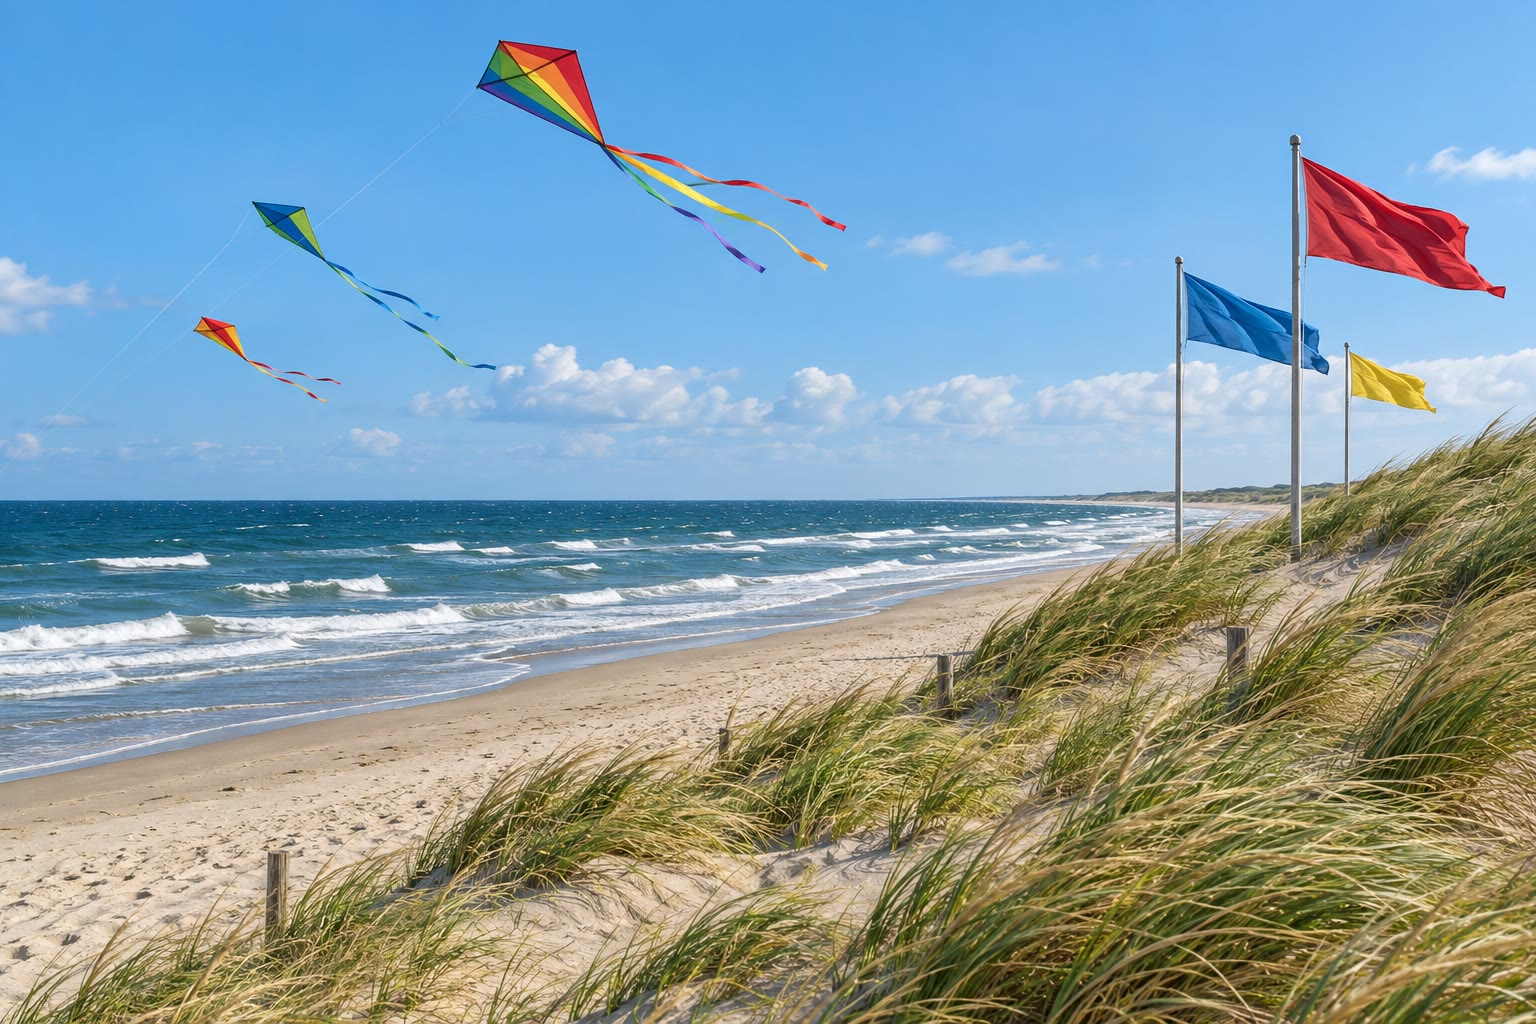
\includegraphics[width=0.55\linewidth]{images/book1/ai/g8-beach-kites.jpg}

{\small किसी \omterm{def:g2:water-on-earth:ocean}{समुद्र} \omterm{def:g1:landscapes-around-us:water}{तट} पर दोपहर बाद की पवन में उड़ती पतंगें (एक सामान्य दृश्य का AI
चित्रण)।}
\label{fig:g8:winds-global-circulation:kites}
\end{omfigure}

\section{वैश्विक पवनें}

यही बात पूरी पृथ्वी के पैमाने पर होती है। \omterm{def:g3:continents-and-oceans:equator}{भूमध्य रेखा} के पास बहुत गरम हुई हवा ऊपर
उठती है; ऊँचाई पर वह \omterm{def:g3:continents-and-oceans:poles}{ध्रुवों} की ओर फैलती है और \ang{30} \omterm{def:g6:latitude-longitude:latitude}{अक्षांश} के पास फिर नीचे
उतरती है। बहुत-से वर्षों के औसत में, हर \omterm{def:g3:continents-and-oceans:equator}{गोलार्ध} का \omterm{def:g8:the-atmosphere:layers}{क्षोभमंडल} तीन बड़े \omterm{def:g8:winds-global-circulation:convection-cell}{संवहन कोष्ठों} में
घूमता है: एक \omterm{def:g3:continents-and-oceans:equator}{भूमध्य रेखा} से लगभग \ang{30} तक, एक लगभग \ang{30} से लगभग \ang{60}
तक, और एक लगभग \ang{60} से \omterm{def:g3:continents-and-oceans:poles}{ध्रुव} तक। मौसम वैज्ञानिक उन्हें हैडली, फ़ेरल और ध्रुवीय
कोष्ठ कहते हैं। उनकी सीमाएँ ऋतुओं के साथ खिसकती हैं, और बीच वाला कोष्ठ गुज़रते हुए
बहुत-से \omterm{def:g5:natural-hazards:storm}{तूफ़ानों} का एक मोटा औसत
है।
% ledger: mo:three-cells, mo:global-circ, nos:doldrums

अगर पृथ्वी न घूमती, तो ज़मीन पर बहने वाली पवनें उच्च से निम्न दाब की ओर सीधी जातीं।
क्योंकि पृथ्वी घूमती है, चलती हवा एक ओर मुड़ जाती है: \omterm{def:g3:continents-and-oceans:equator}{उत्तरी गोलार्ध} में दाईं ओर,
\omterm{def:g3:continents-and-oceans:equator}{दक्षिणी गोलार्ध} में बाईं ओर। इसलिए \omterm{def:g3:continents-and-oceans:equator}{भूमध्य रेखा} की ओर वापस बहने वाली हवा उत्तर से
नहीं आती, बल्कि \omterm{def:g3:continents-and-oceans:equator}{उत्तरी गोलार्ध} में उत्तर-पूर्व से और \omterm{def:g3:continents-and-oceans:equator}{दक्षिणी गोलार्ध} में
दक्षिण-पूर्व से आती है।
% ledger: mo:global-circ, nos:trade-winds

\begin{definition}[वैश्विक पवनें]\label{def:g8:winds-global-circulation:global-winds}
\omterm{def:g6:latitude-longitude:latitude}{अक्षांश} की हर पेटी में ज़मीन पर सबसे अक्सर बहने वाली पवनें हैं:
\begin{itemize}
  \item \emph{व्यापारिक पवनें}\index{व्यापारिक पवनें}, \omterm{def:g3:continents-and-oceans:equator}{भूमध्य रेखा} और लगभग \ang{30}
        के बीच, जो \omterm{def:g3:continents-and-oceans:equator}{उत्तरी गोलार्ध} में उत्तर-पूर्व से और \omterm{def:g3:continents-and-oceans:equator}{दक्षिणी गोलार्ध} में
        दक्षिण-पूर्व से बहती हैं;
  \item \emph{पछुआ पवनें}\index{पछुआ पवनें}, लगभग \ang{30} और \ang{60} के बीच,
        जो पश्चिम से बहती हैं (\omterm{def:g3:continents-and-oceans:equator}{उत्तरी गोलार्ध} में दक्षिण-पश्चिम से, दक्षिणी में
        उत्तर-पश्चिम से);
  \item \emph{ध्रुवीय पुरवा पवनें}\index{ध्रुवीय पुरवा पवनें}, लगभग \ang{60} और
        \omterm{def:g3:continents-and-oceans:poles}{ध्रुवों} के बीच, जो पूर्व से बहती हैं।
\end{itemize}
\end{definition}
% ledger: nos:trade-winds, mo:three-cells, mo:global-circ

\begin{omfigure}
\begin{tikzpicture}[font=\scriptsize, >={Stealth[length=1.8mm]}]
  \def\R{3}
  \fill[blue!8] (0,0) circle (\R);
  \draw (0,0) circle (\R);
  \draw[black!45] (-\R,0) -- (\R,0);
  \foreach \l in {-60,-30,30,60} {
    \pgfmathsetmacro{\y}{\R*sin(\l)}
    \pgfmathsetmacro{\x}{\R*cos(\l)}
    \draw[black!45, dashed] (-\x,\y) -- (\x,\y);}
  % surface winds: NE trades, SW westerlies, NE polar easterlies (north); mirrored south
  \foreach \x in {-1.8,-0.6,0.6,1.8} {
    \draw[->, omThm, line width=0.9pt] (\x+0.35,0.95) -- (\x-0.35,0.55);
    \draw[->, omThm, line width=0.9pt] (\x+0.35,-0.95) -- (\x-0.35,-0.55);}
  \foreach \x in {-1.2,0,1.2} {
    \draw[->, omDef, line width=0.9pt] (\x-0.35,1.7) -- (\x+0.35,2.02);
    \draw[->, omDef, line width=0.9pt] (\x-0.35,-1.7) -- (\x+0.35,-2.02);}
  \foreach \x in {-0.4,0.4} {
    \draw[->, omMeth, line width=0.9pt] (\x+0.25,2.85) -- (\x-0.25,2.65);
    \draw[->, omMeth, line width=0.9pt] (\x+0.25,-2.85) -- (\x-0.25,-2.65);}
  \node[fill=blue!8, inner sep=1pt] at (0,1.2) {उत्तर-पूर्वी व्यापारिक पवनें};
  \node[fill=blue!8, inner sep=1pt] at (0,-1.2) {दक्षिण-पूर्वी व्यापारिक पवनें};
  \node[fill=blue!8, inner sep=1pt] at (0,2.3) {पछुआ पवनें};
  \node[fill=blue!8, inner sep=1pt] at (0,-2.3) {पछुआ पवनें};
  \node[anchor=south] at (0,\R+0.05) {ध्रुवीय पुरवा पवनें};
  \node[anchor=north] at (0,-\R-0.05) {ध्रुवीय पुरवा पवनें};
  % pressure belts on the left
  \foreach \l/\t in {90/{उच्च: उतरती हवा}, 60/{निम्न: उठती हवा}, 30/{उच्च: उतरती हवा, सूखा, मरुस्थल}, 0/{निम्न: उठती हवा, बादल, वर्षा}, -30/{उच्च: उतरती हवा, सूखा, मरुस्थल}, -60/{निम्न: उठती हवा}, -90/{उच्च: उतरती हवा}} {
    \pgfmathsetmacro{\y}{\R*sin(\l)}
    \pgfmathsetmacro{\x}{\R*cos(\l)}
    \draw[black!40] (-\x-0.05,\y) -- (-3.35,\y);
    \node[anchor=east] at (-3.4,\y) {\t};}
  \foreach \l/\t in {60/{\ang{60}~उ}, 30/{\ang{30}~उ}, 0/{भूमध्य रेखा}, -30/{\ang{30}~द}, -60/{\ang{60}~द}} {
    \pgfmathsetmacro{\y}{\R*sin(\l)}
    \pgfmathsetmacro{\x}{\R*cos(\l)}
    \node[anchor=west, black!60] at (\x+0.05,\y) {\t};}
  % side view of the cells (height to the right), same latitude scale
  \begin{scope}[xshift=5.2cm]
    \draw[->] (0,-\R) -- (0,\R+0.3);
    \draw (0,-\R) -- (1.8,-\R);
    \node[anchor=north, align=center] at (0.9,-\R-0.05) {क्षोभमंडल में\\ऊँचाई $\rightarrow$};
    \foreach \lo/\hi/\cw in {0/30/0, 30/60/1, 60/90/0, -30/0/1, -60/-30/0, -90/-60/1} {
      \pgfmathsetmacro{\ya}{\R*sin(\lo)}
      \pgfmathsetmacro{\yb}{\R*sin(\hi)}
      \pgfmathsetmacro{\yc}{(\ya+\yb)/2}
      \pgfmathsetmacro{\bb}{max(0.09,(\yb-\ya)/2-0.06)}
      \ifnum\cw=0
        \draw[black!70, line width=0.7pt, postaction={decorate}, decoration={markings,
          mark=at position 0.125 with {\arrow{Stealth[length=1.6mm]}}, mark=at position 0.375 with {\arrow{Stealth[length=1.6mm]}},
          mark=at position 0.625 with {\arrow{Stealth[length=1.6mm]}}, mark=at position 0.875 with {\arrow{Stealth[length=1.6mm]}}}]
          (0.9,\yc) ++(0.75,0) arc (0:360:0.75 and \bb);
      \else
        \draw[black!70, line width=0.7pt, postaction={decorate}, decoration={markings,
          mark=at position 0.125 with {\arrow{Stealth[length=1.6mm]}}, mark=at position 0.375 with {\arrow{Stealth[length=1.6mm]}},
          mark=at position 0.625 with {\arrow{Stealth[length=1.6mm]}}, mark=at position 0.875 with {\arrow{Stealth[length=1.6mm]}}}]
          (0.9,\yc) ++(0.75,0) arc (360:0:0.75 and \bb);
      \fi}
  \end{scope}
\end{tikzpicture}

{\small \omterm{def:g8:winds-global-circulation:circulation}{वैश्विक परिसंचरण}, सरल रूप में। बाएँ: ज़मीन पर उच्च और निम्न दाब की पेटियाँ।
गोले पर: ज़मीन की पवनें, पृथ्वी के घूमने से एक ओर मुड़ी हुई। दाएँ: हर \omterm{def:g3:continents-and-oceans:equator}{गोलार्ध} के तीन
\omterm{def:g8:winds-global-circulation:convection-cell}{संवहन कोष्ठ}, बगल से देखे गए, उन्हीं \omterm{def:g6:latitude-longitude:latitude}{अक्षांशों} पर (ध्रुवीय कोष्ठ बहुत पतले बनाए गए
हैं क्योंकि गोले पर ध्रुवीय पट्टी संकरी
है)।}
% ledger: mo:three-cells, mo:global-circ, nos:trade-winds, nos:doldrums
\label{fig:g8:winds-global-circulation:cells}
\end{omfigure}

\begin{method}[किसी अक्षांश पर वैश्विक पवन ढूँढना]\label{met:g8:winds-global-circulation:wind}
\begin{enumerate}
  \item पेटी ढूँढो: \omterm{def:g3:continents-and-oceans:equator}{भूमध्य रेखा} से लगभग \ang{30} तक, \ang{30} से \ang{60} तक, या
        \ang{60} से \omterm{def:g3:continents-and-oceans:poles}{ध्रुव} तक।
  \item पता करो कि उस पेटी में ज़मीन पर हवा किस ओर बहती है: पहली और आख़िरी पेटी में
        \omterm{def:g3:continents-and-oceans:equator}{भूमध्य रेखा} की ओर, बीच वाली में \omterm{def:g3:continents-and-oceans:poles}{ध्रुव} की
        ओर।
  \item इस बहाव को एक ओर मोड़ो: \omterm{def:g3:continents-and-oceans:equator}{उत्तरी गोलार्ध} में दाईं ओर, \omterm{def:g3:continents-and-oceans:equator}{दक्षिणी गोलार्ध} में बाईं
        ओर।
  \item बताओ कि पवन कहाँ से आती है: पवनों के नाम उस दिशा पर रखे जाते हैं
        \emph{जहाँ से} वे बहती हैं।
\end{enumerate}
\end{method}

\begin{example}[\ang{40} दक्षिण पर पवन]\label{ex:g8:winds-global-circulation:40s}
\ang{40} दक्षिण पर हम बीच वाली पेटी में हैं, \ang{30} और \ang{60} के बीच। वहाँ
ज़मीन पर हवा \omterm{def:g3:continents-and-oceans:poles}{ध्रुव} की ओर, यानी दक्षिण की ओर, बहती है। \omterm{def:g3:continents-and-oceans:equator}{दक्षिणी गोलार्ध} में वह बाईं ओर
मुड़ती है: दक्षिण जाती हवा के लिए बायाँ पूर्व है, इसलिए हवा आख़िर में दक्षिण-पूर्व की
ओर चलती है। इसलिए वह उत्तर-पश्चिम से आती है: वह \omterm{def:g8:winds-global-circulation:global-winds}{पछुआ पवनों} में से एक है, जो
उत्तर-पश्चिम से बहती
है।
\end{example}
% ledger: mo:three-cells, mo:global-circ

\omterm{def:g3:continents-and-oceans:equator}{भूमध्य रेखा} के पास, जहाँ दोनों \omterm{def:g3:continents-and-oceans:equator}{गोलार्धों} की \omterm{def:g8:winds-global-circulation:global-winds}{व्यापारिक पवनें} मिलती हैं, पवनें थम जाती
हैं: नाविक शांति की इस पेटी को \emph{डोलड्रम} कहते थे। गरम, नम हवा वहाँ ऊपर उठती
है, ठंडी होती है और लगातार बौछारें और तड़ित-झंझा लाती है। \ang{30} के पास, नीचे उतरती
हवा के नीचे, पवनें हल्की होती हैं और वर्षा दुर्लभ होती
है।
% ledger: nos:doldrums

\begin{definition}[वायुमंडल का वैश्विक परिसंचरण]\label{def:g8:winds-global-circulation:circulation}
वायुमंडल का \emph{वैश्विक परिसंचरण}\index{वैश्विक परिसंचरण} पूरे ग्रह के चारों ओर
हवा की बड़े पैमाने की गति है, जो बहुत-से वर्षों की पवनों का औसत लेने पर दिखती है। यह
ऊष्मा को \omterm{def:g3:continents-and-oceans:equator}{भूमध्य रेखा} से \omterm{def:g3:continents-and-oceans:poles}{ध्रुवों} की ओर, और जलवाष्प को \omterm{def:g6:latitude-longitude:latitude}{अक्षांश} की एक पेटी से दूसरी
पेटी तक ले जाता
है।
\end{definition}
% ledger: mo:global-circ

\section{वैश्विक परिसंचरण और जलवायु क्षेत्र}

\omterm{def:g8:winds-global-circulation:circulation}{वैश्विक परिसंचरण} \omterm{def:g5:weather-and-climate:climate}{जलवायु} के \omterm{def:g2:drawing-to-map:map}{मानचित्र} का बहुत-सा हिस्सा समझाता है। जहाँ हवा ऊपर उठती है,
\omterm{def:g3:continents-and-oceans:equator}{भूमध्य रेखा} के पास, वह ठंडी होती है और उसकी जलवाष्प \omterm{def:g4:clouds-rain-snow:cloud}{बादलों} में बदल जाती है: वर्षा
अक्सर होती है, और \omterm{def:g5:weather-and-climate:rainforest}{वर्षावन} उगते हैं। जहाँ हवा नीचे उतरती है, \ang{30} उत्तर और
दक्षिण के पास, वह नीचे आते हुए गरम होती है, उसके \omterm{def:g4:clouds-rain-snow:cloud}{बादल} सूख जाते हैं, और वर्षा दुर्लभ
होती है: सहारा जैसे बड़े गरम \omterm{def:g5:weather-and-climate:desert}{मरुस्थल} इन्हीं पेटियों में हैं। मध्य \omterm{def:g6:latitude-longitude:latitude}{अक्षांशों} में \omterm{def:g8:winds-global-circulation:global-winds}{पछुआ
पवनें} एक के बाद एक \omterm{def:g5:natural-hazards:storm}{तूफ़ान} लाती हैं, हर ऋतु में वर्षा के
साथ।
% ledger: nos:doldrums, mo:three-cells, mo:global-circ

\begin{omfigure}
\begin{minipage}[c]{0.42\linewidth}\centering
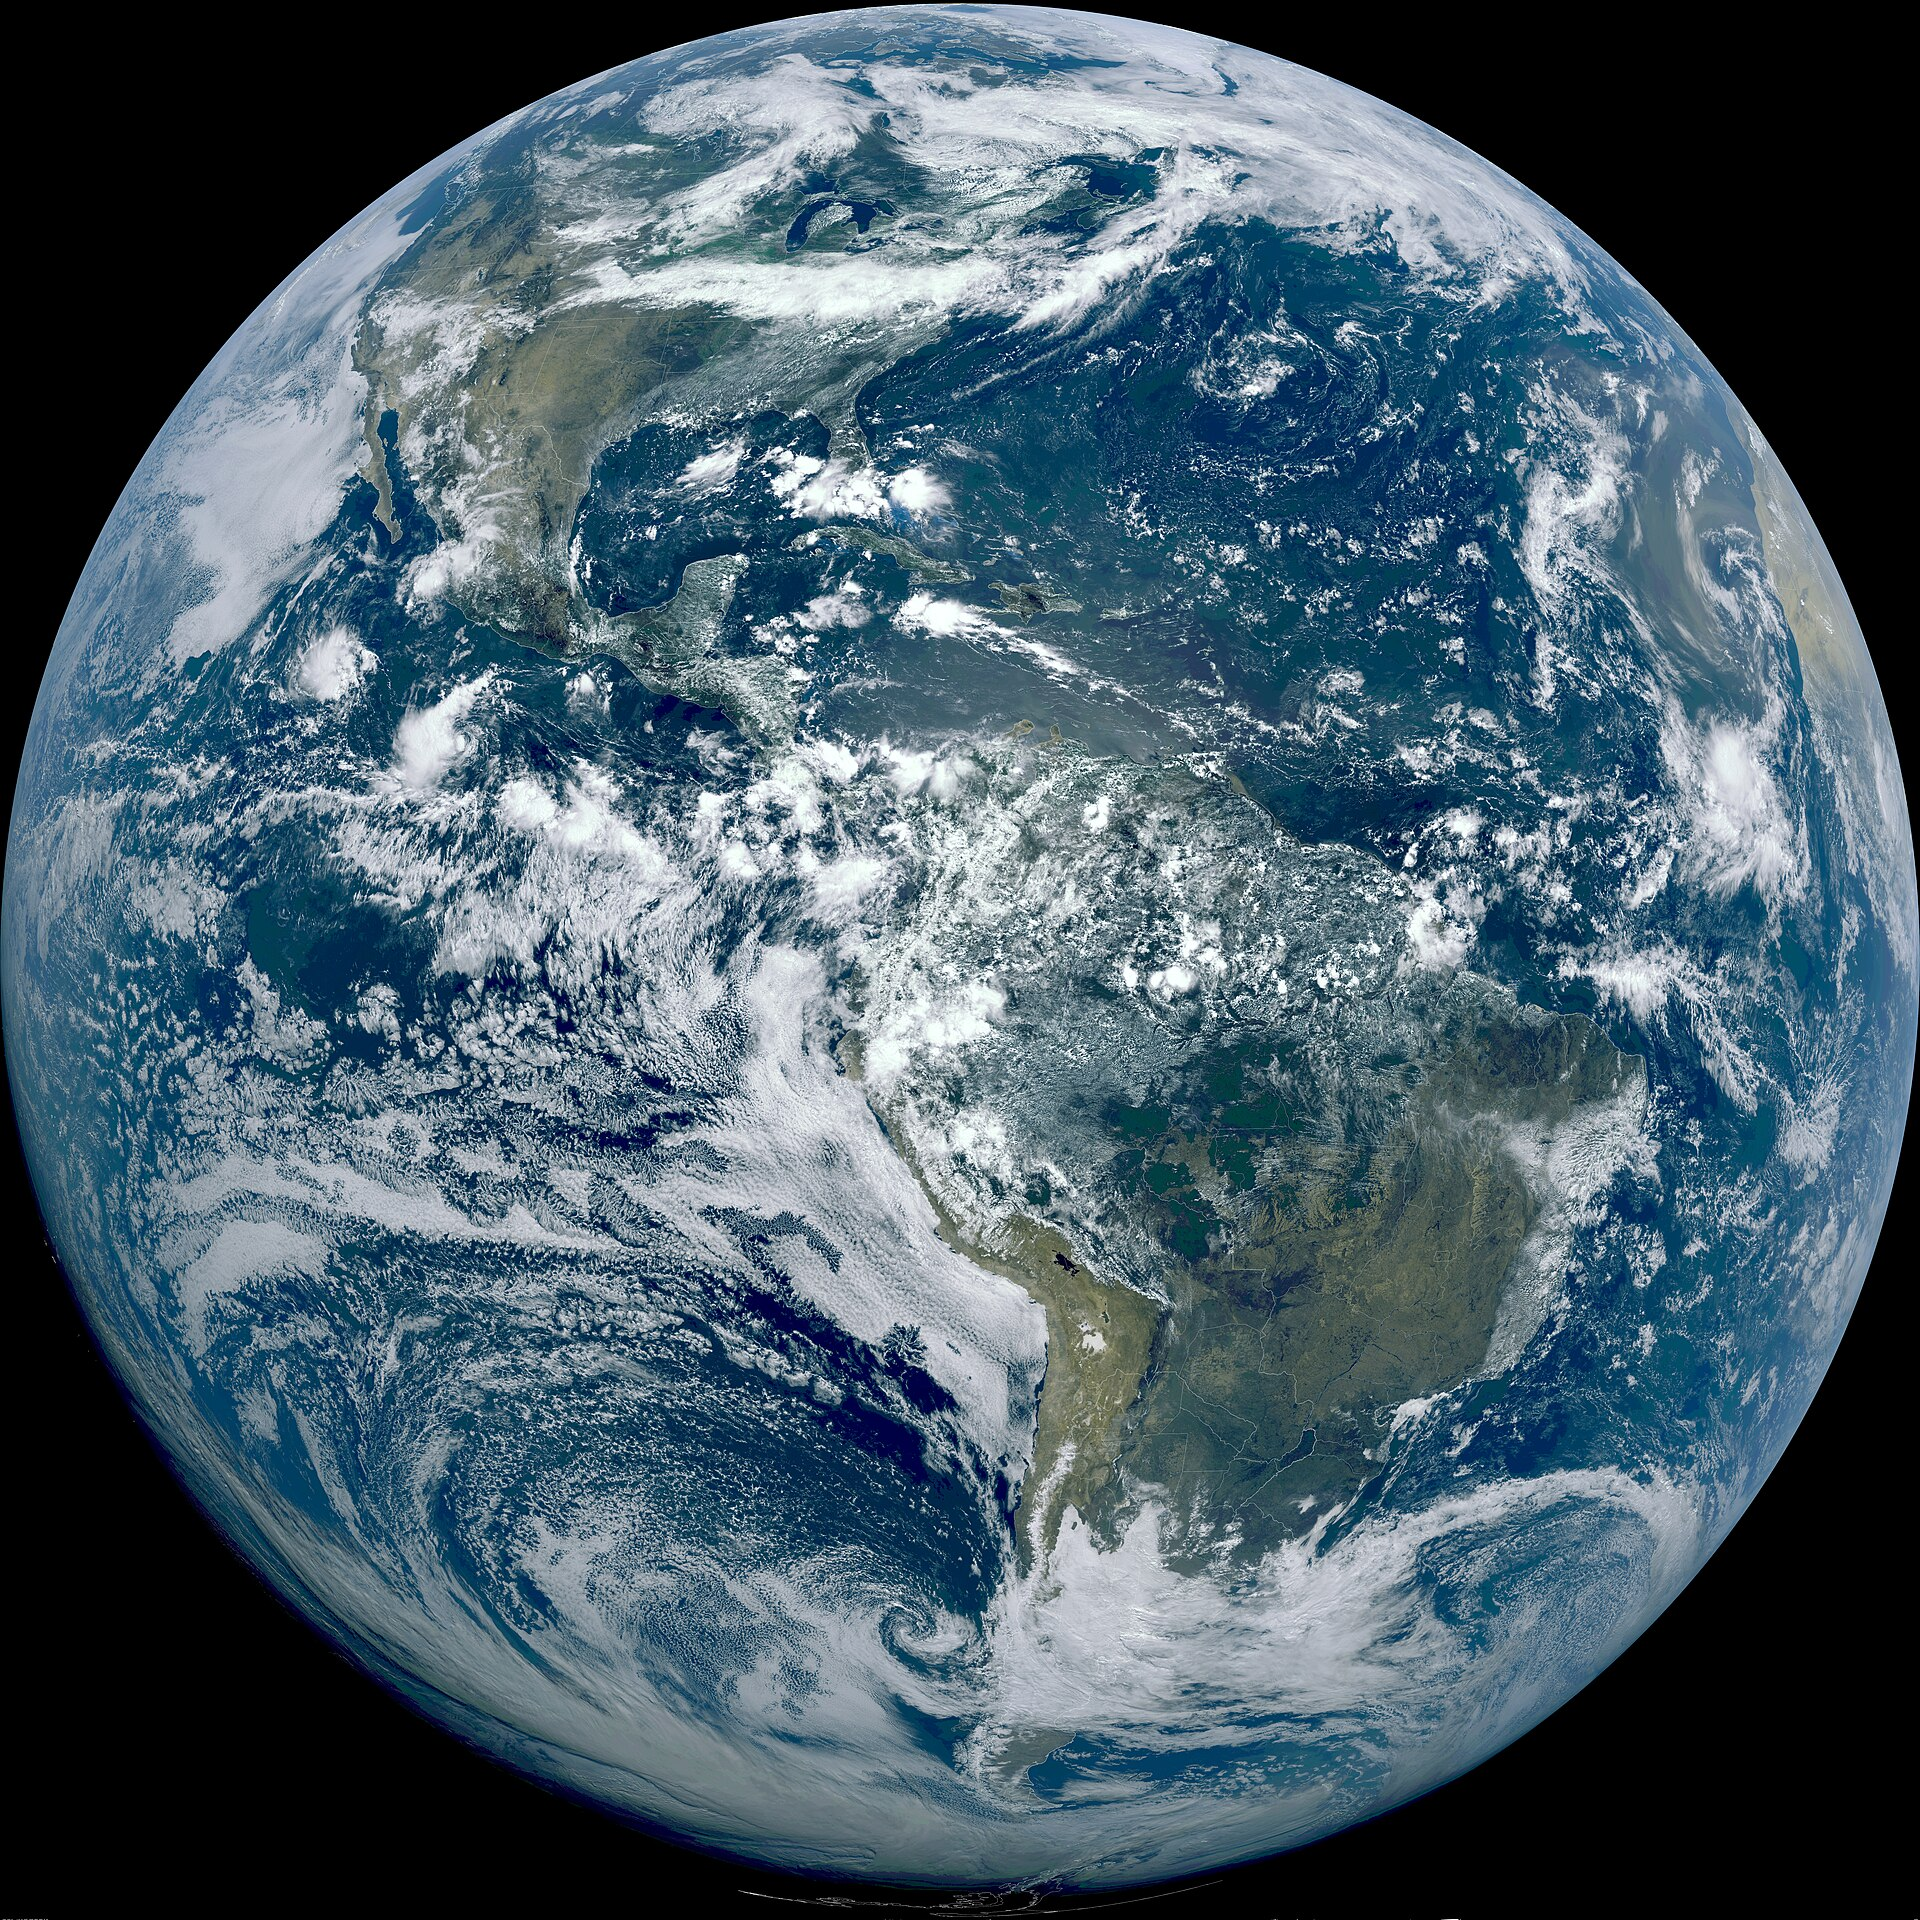
\includegraphics[width=\linewidth]{images/book1/g8-goes-full-disk.jpg}
\end{minipage}\hfill
\begin{minipage}[c]{0.54\linewidth}\raggedright
{\small \omterm{def:g3:continents-and-oceans:equator}{भूमध्य रेखा} के बहुत ऊपर स्थित \omterm{def:g1:watching-the-weather:weather}{मौसम} उपग्रह GOES-16 से 26~जुलाई 2022 को देखे
गए अमेरिका \omterm{def:g3:continents-and-oceans:continent}{महाद्वीप}। \omterm{def:g5:weather-and-climate:tropics}{कर्क और मकर रेखाओं} के बीच के क्षेत्र और अमेज़न \omterm{def:g5:weather-and-climate:rainforest}{वर्षावन} के ऊपर,
जहाँ गरम, नम हवा ऊपर उठती है, बहुत-से \omterm{def:g4:clouds-rain-snow:cloud}{बादल} बने हैं; दूर दक्षिण में, दक्षिणी जाड़े
में, \omterm{def:g8:winds-global-circulation:global-winds}{पछुआ पवनों} के \omterm{def:g5:natural-hazards:storm}{तूफ़ान} \omterm{def:g2:water-on-earth:ocean}{महासागर} के ऊपर घूमते हैं। NOAA (सार्वजनिक डोमेन,
विकिमीडिया कॉमन्स के ज़रिए)।}
\end{minipage}
% ledger: commons:goes16, nos:doldrums
\label{fig:g8:winds-global-circulation:goes}
\end{omfigure}

\begin{example}[चार शहर, चार पेटियाँ]\label{ex:g8:winds-global-circulation:four-towns}
\cref{ch:g5:weather-and-climate} के \omterm{def:g5:weather-and-climate:climate}{जलवायु} चार्टों वाले चारों शहर \omterm{def:g3:continents-and-oceans:equator}{उत्तरी गोलार्ध} में,
बहुत अलग-अलग \omterm{def:g6:latitude-longitude:latitude}{अक्षांशों} पर हैं। उनकी वार्षिक वर्षा और \omterm{def:g4:clouds-rain-snow:precipitation}{हिम} \omterm{def:g8:winds-global-circulation:circulation}{वैश्विक परिसंचरण} की पेटियों
के अनुसार हैं (नीचे का चार्ट)। हिलो, \ang{20} उत्तर पर, \omterm{def:g8:winds-global-circulation:global-winds}{व्यापारिक पवनों} की पेटी में
\omterm{def:g2:water-on-earth:ocean}{महासागर} के बीच एक द्वीप पर है, जहाँ \omterm{def:g8:winds-global-circulation:global-winds}{व्यापारिक पवनें} जलवाष्प उठाती हैं: वहाँ एक वर्ष
में लगभग \qty{3000}{mm} गिरता है। फ़ीनिक्स, \ang{33} उत्तर पर, \ang{30} के पास,
नीचे उतरती हवा के नीचे है: \qty{200}{mm} से कम। सिएटल, \ang{47} उत्तर पर, \omterm{def:g8:winds-global-circulation:global-winds}{पछुआ
पवनों} में है, जिनके \omterm{def:g5:natural-hazards:storm}{तूफ़ान} एक वर्ष में लगभग \qty{1000}{mm} लाते हैं, उसका
ज़्यादातर हिस्सा पतझड़ से वसंत तक। उत्कियाग्विक, \ang{71} उत्तर पर, उस ठंडी हवा के
नीचे है जो \omterm{def:g3:continents-and-oceans:poles}{ध्रुव} के पास नीचे उतरती है: \qty{150}{mm} से कम, एक ठंडा
\omterm{def:g5:weather-and-climate:desert}{मरुस्थल}।
% ledger: data:b1-noaa-normals (totals from figdata/grade-5/climate_charts.py, re-read in figdata/grade-8/rain_by_belt.py), mo:three-cells, nos:doldrums
\end{example}

\begin{omfigure}
\begin{tikzpicture}
\begin{axis}[xbar, width=0.82\linewidth, height=6.4cm, bar width=9pt,
  xmin=0, xmax=3600, ymin=0, ymax=90, ytick={0,30,60,90},
  yticklabels={$0^\circ$, $30^\circ$\,उ, $60^\circ$\,उ, $90^\circ$\,उ},
  xlabel={एक वर्ष में वर्षा और हिम (mm)}, ylabel={अक्षांश},
  axis x line=bottom, axis y line=left, axis line style={-},
  tick label style={font=\scriptsize}, label style={font=\small},
  xtick={0,1000,2000,3000}, scaled x ticks=false, clip=false,
  ]
  \draw[black!35, dashed] (axis cs:0,30) -- (axis cs:3600,30);
  \draw[black!35, dashed] (axis cs:0,60) -- (axis cs:3600,60);
  \node[font=\scriptsize, black!60, anchor=south east] at (axis cs:3600,1) {उठती हवा: वर्षा};
  \node[font=\scriptsize, black!60, anchor=south east] at (axis cs:3600,30) {उतरती हवा: सूखा};
  \node[font=\scriptsize, black!60, anchor=south east] at (axis cs:3600,60) {उठती हवा: वर्षा};
  \node[font=\scriptsize, black!60, anchor=north east] at (axis cs:3600,90) {उतरती हवा: सूखा};
  \addplot[fill=blue!35, draw=blue!60!black] table[x=total_mm, y=lat] {figdata/out/grade-8-rain_by_belt-stations.dat};
  \node[font=\scriptsize, anchor=west] at (axis cs:3058,19.72) {हिलो};
  \node[font=\scriptsize, anchor=west] at (axis cs:183,33.43) {फ़ीनिक्स};
  \node[font=\scriptsize, anchor=west] at (axis cs:999,47.44) {सिएटल};
  \node[font=\scriptsize, anchor=west] at (axis cs:137,71.28) {उत्कियाग्विक};
\end{axis}
\end{tikzpicture}

{\small \omterm{def:g5:weather-and-climate:climate}{जलवायु} चार्टों वाले चार शहरों की वार्षिक वर्षा और \omterm{def:g4:clouds-rain-snow:precipitation}{हिम} (1991--2020 के औसत),
उनके \omterm{def:g6:latitude-longitude:latitude}{अक्षांशों} पर रखे गए। नम शहर वहाँ हैं जहाँ हवा ऊपर उठती है, \omterm{def:g3:continents-and-oceans:equator}{भूमध्य रेखा} के पास
और \ang{60} के पास; सूखे शहर वहाँ जहाँ वह नीचे उतरती है, \ang{30} के पास और \omterm{def:g3:continents-and-oceans:poles}{ध्रुव}
के पास। NOAA \omterm{def:g5:weather-and-climate:climate}{जलवायु} सामान्य मान।}
% ledger: data:b1-noaa-normals, mo:three-cells (figdata/grade-8/rain_by_belt.py)
\end{omfigure}

चार शहर केवल चार बिंदु हैं: पहाड़, \omterm{def:g1:landscapes-around-us:water}{तट} और ठंडे या गरम \omterm{def:g2:water-on-earth:ocean}{समुद्र} भी बदलते हैं कि किसी जगह
कितनी वर्षा होती है। पेटियाँ \omterm{def:g5:weather-and-climate:climate}{जलवायु} के \omterm{def:g2:drawing-to-map:map}{मानचित्र} का मोटा ढाँचा देती हैं, हर शहर की
वर्षा नहीं।

\section{अभ्यास}

\begin{exercise}[$\star$]\label{exo:g8:winds-global-circulation:1}
उस वैश्विक पवन का नाम बताओ जो सबसे अक्सर बहती है: (क) \ang{15} उत्तर पर;
(ख) \ang{45} दक्षिण पर; (ग) \ang{75} उत्तर पर; (घ) \ang{20} दक्षिण पर।
हर बार उसकी दिशा बताओ।
\end{exercise}

\begin{exercise}[$\star$]\label{exo:g8:winds-global-circulation:2}
हर वाक्य पूरा करो। (क) गरम हवा \dots\ और ठंडी हवा \dots। (ख) ऊपर उठती हवा के
नीचे ज़मीन पर दाब \dots\ होता है। (ग) ज़मीन पर पवन \dots\ दाब से \dots\ दाब की ओर
बहती है। (घ) \omterm{def:g3:continents-and-oceans:equator}{उत्तरी गोलार्ध} में पृथ्वी का घूमना चलती हवा को \dots\ ओर मोड़ता
है।
\end{exercise}

\begin{exercise}[$\star$]\label{exo:g8:winds-global-circulation:3}
सही या ग़लत? ग़लत वाक्यों को सुधारो। (क) \omterm{def:g8:winds-global-circulation:breezes}{समुद्र समीर} ज़मीन से \omterm{def:g2:water-on-earth:ocean}{समुद्र} की ओर बहता है।
(ख) दिन में ज़मीन \omterm{def:g2:water-on-earth:ocean}{समुद्र} से जल्दी गरम होती है। (ग) \omterm{def:g8:winds-global-circulation:global-winds}{व्यापारिक पवनें} पश्चिम से बहती
हैं। (घ) बहुत-से बड़े \omterm{def:g5:weather-and-climate:desert}{मरुस्थल} \ang{30} \omterm{def:g6:latitude-longitude:latitude}{अक्षांश} के पास
हैं।
\end{exercise}

\begin{exercise}[$\star$]\label{exo:g8:winds-global-circulation:4}
एक \omterm{def:g1:landscapes-around-us:water}{तट} बनाओ, बाईं ओर \omterm{def:g2:water-on-earth:ocean}{समुद्र} और दाईं ओर ज़मीन। सूर्य जोड़ो, फिर तीरों से \omterm{def:g8:winds-global-circulation:breezes}{समुद्र समीर}
का हवा का चक्कर बनाओ। जहाँ ज़मीन पर दाब उच्च और निम्न है, वहाँ उच्च और निम्न
लिखो।
\end{exercise}

\begin{exercise}[$\star\star$]\label{exo:g8:winds-global-circulation:5}
इस अध्याय की पुंजों वाली तालिका का उपयोग करो। (क) \ang{45} पर एक पुंज \omterm{def:g3:continents-and-oceans:equator}{भूमध्य रेखा}
की तुलना में कितनी ज़्यादा ज़मीन ढकता है? (ख) \ang{60} पर हर वर्ग मीटर को \omterm{def:g3:continents-and-oceans:equator}{भूमध्य
रेखा} की ऊर्जा का कितना प्रतिशत मिलता है? (ग) \ang{75} पर? (घ) एक वाक्य में समझाओ
कि \omterm{def:g3:continents-and-oceans:poles}{ध्रुव} ठंडे क्यों हैं।
\end{exercise}

\begin{exercise}[$\star\star$]\label{exo:g8:winds-global-circulation:6}
एक नाव \omterm{def:g3:continents-and-oceans:equator}{उत्तरी गोलार्ध} और फिर \omterm{def:g3:continents-and-oceans:equator}{दक्षिणी गोलार्ध} से होकर ठीक दक्षिण की ओर चलती है।
(क) \ang{70} उत्तर से \ang{70} दक्षिण तक, क्रम से, उसे कौन-सी पवनें मिलती हैं? (ख) उसे शांत
हवा और लगातार बौछारें कहाँ मिलने की संभावना है? (ग) पवनें कहाँ हल्की और वर्षा
दुर्लभ हैं?
\end{exercise}

\begin{exercise}[$\star\star$]\label{exo:g8:winds-global-circulation:7}
एक \omterm{def:g2:water-on-earth:ocean}{समुद्र} \omterm{def:g1:landscapes-around-us:water}{तट} पर दोपहर 3~बजे \omterm{def:g3:stones-pebbles-sand:sand}{रेत} पर \qty{31}{\degreeCelsius} और \omterm{def:g2:water-on-earth:ocean}{समुद्र} के ऊपर
\qty{22}{\degreeCelsius} है। रात 3~बजे ज़मीन पर \qty{17}{\degreeCelsius} और
\omterm{def:g2:water-on-earth:ocean}{समुद्र} के ऊपर \qty{21}{\degreeCelsius} है। (क) दोपहर 3~बजे कौन ज़्यादा गरम है? पवन
किस ओर बहती है? (ख) और रात 3~बजे? (ग) दोनों समयों के बीच ज़मीन का तापमान कितने
डिग्री बदलता है? और \omterm{def:g2:water-on-earth:ocean}{समुद्र} का तापमान? (घ) अंतर
समझाओ।
\end{exercise}

\begin{exercise}[$\star\star$]\label{exo:g8:winds-global-circulation:8}
हवा \ang{30} उत्तर के पास की उच्च दाब पेटी से \omterm{def:g3:continents-and-oceans:equator}{भूमध्य रेखा} की ओर बहती है। (क) पृथ्वी के
घूमने के बिना वह किस दिशा से बहती? (ख) इस \omterm{def:g3:continents-and-oceans:equator}{गोलार्ध} में घूमना उसे किस ओर मोड़ता है?
(ग) तब वह किस दिशा से बहती है? (घ) \ang{30} दक्षिण से \omterm{def:g3:continents-and-oceans:equator}{भूमध्य रेखा} की ओर बहती हवा के लिए
यही तीन प्रश्न हल
करो।
\end{exercise}

\begin{exercise}[$\star\star$]\label{exo:g8:winds-global-circulation:9}
क़दम-दर-क़दम समझाओ कि \omterm{def:g3:continents-and-oceans:equator}{भूमध्य रेखा} के पास इतनी अक्सर वर्षा क्यों होती है: ये शब्द
इस्तेमाल करो: \emph{गरम होती है}, \emph{ऊपर उठती है}, \emph{ठंडी होती है},
\emph{\omterm{def:g4:clouds-rain-snow:cloud}{बादल}}। फिर समझाओ कि उत्तरी अफ़्रीका में \ang{25} उत्तर के पास \omterm{def:g5:weather-and-climate:desert}{मरुस्थल} क्यों है: ये
शब्द इस्तेमाल करो: \emph{नीचे उतरती है}, \emph{उच्च दाब}, \emph{सूखा}।
\end{exercise}

\begin{exercise}[$\star\star$]\label{exo:g8:winds-global-circulation:10}
एक पाल-जहाज़ यूरोप के पश्चिमी \omterm{def:g1:landscapes-around-us:water}{तट} पर \ang{40} उत्तर के एक बंदरगाह से कैरिबियन के लिए,
\ang{15} उत्तर पर, निकलता है। (क) \ang{40} उत्तर पर उसे कौन-सी पवन मिलेगी? क्या वह जहाज़
को पश्चिम की ओर चलने में मदद करेगी? (ख) जहाज़ को पहले दक्षिण की ओर क्यों चलना
चाहिए? (ग) कौन-सी पवन उसे पश्चिम की ओर ले जाती है, और किन \omterm{def:g6:latitude-longitude:latitude}{अक्षांशों} के बीच?
(घ) यूरोप लौटने की यात्रा के लिए जहाज़ को कौन-सी पवन ढूँढनी चाहिए, और किस \omterm{def:g6:latitude-longitude:latitude}{अक्षांश}
पर?
\end{exercise}

\begin{exercise}[$\star\star\star$]\label{exo:g8:winds-global-circulation:11}
\omterm{def:g6:latitude-longitude:latitude}{अक्षांश} $L$ पर, किसी विषुव के दिन दोपहर को सूर्य के प्रकाश का एक पुंज \omterm{def:g3:continents-and-oceans:equator}{भूमध्य रेखा} पर
ढकी ज़मीन का $1 \div
\cos L$ गुना ढकता है (कैलकुलेटर पर, $\cos 60^\circ = 0.5$)।
(क) \ang{60} का मान जाँचो। (ख) $\cos 30^\circ \approx 0.866$ का उपयोग करके,
\ang{30} का मान जाँचो, दो दशमलव स्थानों तक पूर्णांकित। (ग) मान लो समतल रखा एक सौर
पैनल उस दिन \omterm{def:g3:continents-and-oceans:equator}{भूमध्य रेखा} पर दोपहर को हर वर्ग मीटर पर \qty{1000}{W} पाता है। वही
पैनल \ang{30} पर लगभग कितना पाएगा? \ang{60} पर?
\end{exercise}

\begin{exercise}[$\star\star\star$]\label{exo:g8:winds-global-circulation:12}
हर \omterm{def:g3:continents-and-oceans:equator}{गोलार्ध} में \omterm{def:g8:winds-global-circulation:circulation}{वैश्विक परिसंचरण} के तीन कोष्ठ हैं। (क) \omterm{def:g3:continents-and-oceans:equator}{उत्तरी गोलार्ध} का बगल से दृश्य
बनाओ, नीचे \omterm{def:g3:continents-and-oceans:equator}{भूमध्य रेखा} और ऊपर \omterm{def:g3:continents-and-oceans:poles}{ध्रुव}, और तीनों कोष्ठ चक्करों के रूप में; दिखाओ कि हवा
कहाँ ऊपर उठती है और कहाँ नीचे उतरती है। (ख) ज़मीन पर उच्च और निम्न दाब की पेटियाँ
चिह्नित करो। (ग) हर कोष्ठ की ज़मीनी पवनें जोड़ो, दाईं ओर मुड़ी हुई। (घ) अपने चित्र
का उपयोग करके समझाओ कि \omterm{def:g8:winds-global-circulation:global-winds}{पछुआ पवनें} उत्तर-पूर्व की ओर क्यों बहती
हैं।
\end{exercise}

\section{समस्या: व्यापारिक पवनों के साथ नौकायन}

\begin{problem}[{सप्ताहांत समस्या --- एक पाल-जहाज़ उत्तर-पूर्वी व्यापारिक पवन के साथ
काबो वर्दे से बारबाडोस तक अटलांटिक पार करता है; मानचित्र पर रास्ता मापा जाता है, पवन
पढ़ी जाती है, और यात्रा की अवधि निकाली
जाती है}]
\label{pb:g8:winds-global-circulation:1}
% ledger: data:b1-ne-places, earth:Rmean, nos:trade-winds (figdata/grade-8/trade_route.py; the speed is exercise data)
एक पाल-जहाज़ काबो वर्दे द्वीपों के प्राइया से बारबाडोस के ब्रिजटाउन के लिए निकलता है।
\omterm{def:g2:drawing-to-map:map}{मानचित्र} रास्ता और व्यापारिक पवन दिखाता है।

\begin{center}
\begin{tikzpicture}
\begin{axis}[ommap, width=12cm, xmin=-75, xmax=-5, ymin=0, ymax=35, axis equal image,
  xtick={-70,-60,-50,-40,-30,-20,-10}, ytick={0,10,20,30},
  tick label style={font=\scriptsize},
  xlabel={देशांतर (ऋणात्मक = पश्चिम)}, ylabel={अक्षांश (उत्तर)},
  label style={font=\small}, clip mode=individual]
  \addplot[fill=omLithAlluv, draw=black!60, line width=0.3pt] table {figdata/out/grade-8-trade_route-land.dat};
  \addplot[quiver={u=\thisrow{dlon}, v=\thisrow{dlat}}, -{Stealth[length=1.6mm]}, omThm!80, line width=0.7pt]
    table[x=lon, y=lat] {figdata/out/grade-8-trade_route-trades.dat};
  \addplot[omDef, line width=1.3pt, dashed] table {figdata/out/grade-8-trade_route-route.dat};
  \addplot[only marks, mark=*, mark size=2pt, black] table[x=lon, y=lat] {figdata/out/grade-8-trade_route-ports.dat};
  \node[anchor=north, font=\scriptsize\bfseries, fill=white, inner sep=1pt] at (axis cs:-59.6,12.2) {ब्रिजटाउन};
  \node[anchor=south, font=\scriptsize\bfseries, fill=white, inner sep=1pt] at (axis cs:-23.5,15.8) {प्राइया};
\end{axis}
\end{tikzpicture}
\end{center}

\noindent\textbf{भाग I --- रास्ता।}\par\nopagebreak
\begin{enumerate}[beginpenalty=10000]
  \item प्राइया \ang{14.9} उत्तर, \ang{23.5} पश्चिम पर है; ब्रिजटाउन \ang{13.1} उत्तर,
        \ang{59.6} पश्चिम पर। उन्हें \omterm{def:g6:latitude-longitude:longitude}{देशांतर} के कितने डिग्री अलग करते
        हैं?
  \item दोनों बंदरगाह \ang{14} उत्तर के पास हैं। इस \omterm{def:g6:latitude-longitude:latitude}{अक्षांश रेखा} के साथ, \omterm{def:g6:latitude-longitude:longitude}{देशांतर} का एक
        डिग्री लगभग \qty{108}{km} मापता है। यात्रा लगभग कितने किलोमीटर की है? निकटतम
        सौ तक पूर्णांकित करो।
  \item गोल पृथ्वी पर ठीक-ठीक मापने पर सबसे छोटा रास्ता \qty{3896}{km} है। क्या
        प्रश्न 2 का जवाब एक अच्छा अनुमान है?
  \item क्या बंदरगाह \omterm{def:g8:winds-global-circulation:global-winds}{व्यापारिक पवनों} की पेटी में हैं? समझाओ।
\end{enumerate}

\noindent\textbf{भाग II --- पवन।}\par\nopagebreak
\begin{enumerate}[resume, beginpenalty=10000]
  \item यहाँ व्यापारिक पवन किस दिशा से बहती है?
  \item जहाज़ पश्चिम की ओर चलता है। पवन उसे आगे, पीछे या बगल की ओर धकेलती है?
        \omterm{def:g2:drawing-to-map:map}{मानचित्र} से समझाओ।
  \item यात्रा के लगभग हर दिन व्यापारिक पवन एक ही दिशा में क्यों बहती
        है?
  \item यूरोप लौटते हुए कप्तान को \ang{14} उत्तर के साथ-साथ पूर्व की ओर चलने की कोशिश
        क्यों नहीं करनी चाहिए?
\end{enumerate}

\noindent\textbf{भाग III --- यात्रा।}\par\nopagebreak
\begin{enumerate}[resume, beginpenalty=10000]
  \item मान लो जहाज़ औसतन \qty{7}{km} प्रति घंटा चलता है। 24 घंटे के एक दिन में वह
        कितने किलोमीटर तय करता है?
  \item अगर रास्ते में 3 दिन पवन थम जाए, तो जहाज़ कितने किलोमीटर की प्रगति
        खोएगा?
  \item स्थिर व्यापारिक पवन के साथ जहाज़ को \qty{3896}{km} के लिए कितने दिन चाहिए?
        एक दशमलव स्थान तक पूर्णांकित करो।
  \item निकटतम पूरे दिन तक, यात्रा कितनी देर चलती है? यह एक महीने से ज़्यादा है
        या कम?
\end{enumerate}
\end{problem}
